\documentclass[10pt]{beamer}
\usepackage[slovene]{babel}
\usepackage[utf8]{inputenc}
\usepackage[T1]{fontenc}
\usepackage{amsmath}
\usepackage{eurosym}
\usepackage{amsfonts}
\usepackage{lmodern}
\usepackage{mathptmx}
\usepackage{helvet}
\usepackage{courier}
\usepackage{hyperref}
\usepackage{graphicx}
\usepackage{tikz}
\usepackage{enumerate}
\usetheme{CambridgeUS}
\useoutertheme{infolines} 
\setbeamertemplate{caption}[numbered]


\begin{document}

\title[Proračun Republike Slovenije]{Proračun Republike Slovenije}
\author{Eva Deželak, Žan Jarc, Ines Šilc}
\institute [FMF]{ Fakulteta za matematiko in fiziko}

\newcounter{stevec}

\begin{frame}
	\titlepage
\end {frame}

\begin{frame}
	\frametitle{Vsebina predstavitve}
	\tableofcontents
\end {frame}

\begin{frame}
\section[Splošno o proračunu RS]{Splošno o proračunu RS}
\frametitle{Splošno o proračunu RS}
\begin{itemize}
\item Pripravi ga vlada RS.
\item Sprejme ga Državni zbor.
\item Temeljne naloge: 
\begin{itemize}
\item uresničitev proračuna v okvirih in za namene, kot je bil sprejet
\item njegovo pravočasno in fleksibilno prilagajanjes premenjenim fiskalnim okoliščinam
\item uresničevanje v proračunu zastavljenih družbenih in gospodarskih ciljev.
\end{itemize}
\item Sprejemata se proračuna za dve leti, (t+1) in (t+2).
\end{itemize}
\end{frame}

\begin{frame}
\subsection[Deitev propračuna]{Delitev proračuna}
\frametitle{Delitev proračuna}
	\begin{itemize}
	\item \textbf{Splošni del proračuna:}
		\begin{itemize}
		\item \underline{Bilanca prihodkov in odhodkov} (na strani prihodkov: tekoči prihodki, kapitalski prihodki, prejete donacije in trasferni prihodki iz drugih blagajn javnega financiranja; na strani odhodkov: tekoči odhodki, tekoči transferji, investicijski odhodki in investicijski transferji)
		\item \underline{Račun finančnih terjatev} (na strani izdatkov: tokovi izdatkov, ki za državo nimajo značaja odhodkov - dana posojila finančnih naložb oz. kapitalskih vlog države v javna in zasebna podjetja, banke, itd. ; na strani prejemkov: tokovi prejemkov, ki nimaja značaja prihodkov - sredstva iz naslova prejetih vračil posojenih sredstev države oz. prejeta sredstva iz naslova prodaje kapitalskih deležev države v podjetjih, bankah, itd.)
		\item \underline{Račun financiranja} (tokovi zadolževanja in odplačil dolgov, povezanih s financiranjem proračunskega deficita)
		\end{itemize}
	\item \textbf{Posebni del proračuna:} odhodki in drugi izdatki predstavljeni po politikah, glavnih programih in podprogramih.
	\item \textbf{Načrt razvojnih programov:} odhodki se načrtujejo po strukturi programske klasifikacije, posameznih ukrepih in projektih ter virih financiranja po  posameznih letih za celovito izvedbo projektov in ukrepov.
	\end{itemize}
\end{frame}

\begin{frame}
	\section[Analiza nekaterih sprememb proračuna v letih od 2015 do 2019]{Analiza nekaterih sprememb proračuna v letih od 2015 do 2019}
	\subsection[Davki na premičnine in nepremičnine]{Davki na premičnine in nepremičnine}
	\frametitle{Davki na premičnine in nepremičnine}
	Davek na nepremičnine je bil uveden samo v letu 2015. Istega leta so bili tudi najvišji prihodki iz davka na finančno premoženje in davka na premičnine.
	\begin{figure}[h!]
	\centering
	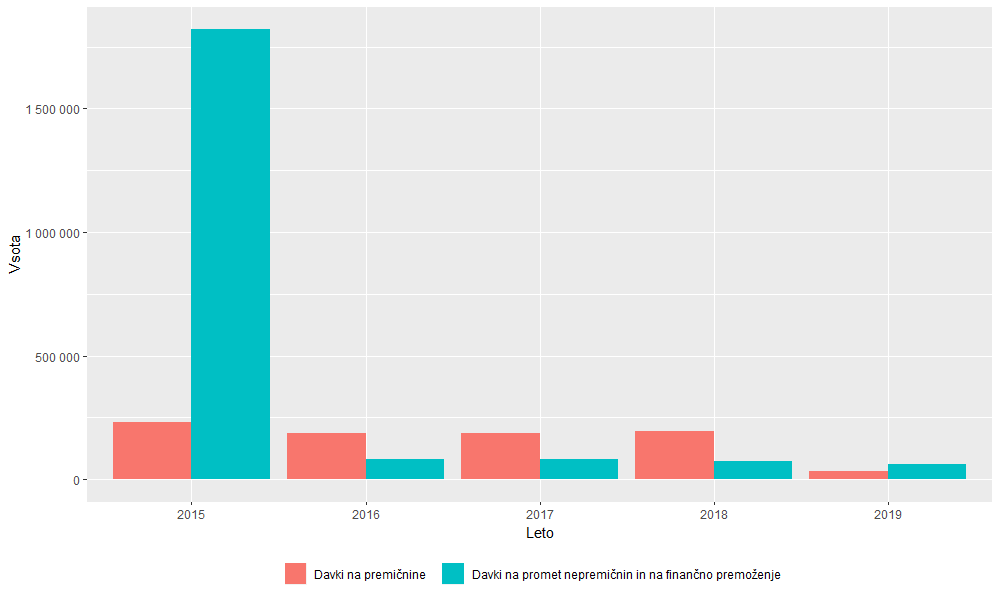
\includegraphics[width = 10 cm]{davki_na_premozenje_graf.png}
	\caption{Prispevki davkov na premičnine in na promet nepremičnin}
	\label{Slika 1}
	\end{figure}
\end {frame}

\begin{frame}
	\subsection[DDPO in dohodnina]{DDPO in dohodnina}
	\frametitle{DDPO in dohodnina}
	\begin{figure}[h!]
	\centering
	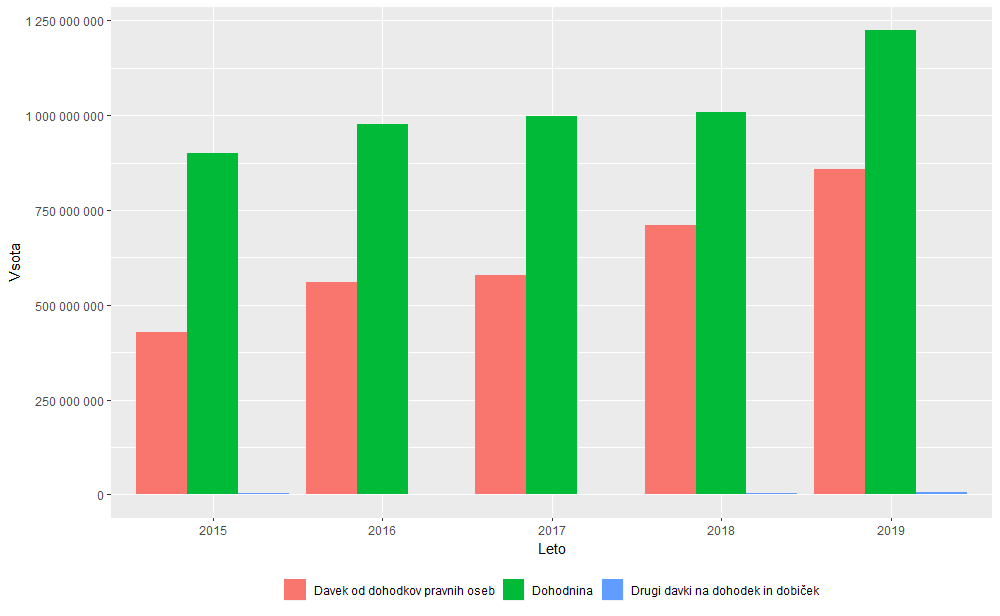
\includegraphics[width = 10 cm]{davki_na_dohodek_in_dobicek_graf.png}
	\caption{Prispevki davkov na dohodek in dobiček}
	\label{Slika 2}
	\end{figure}
\end {frame}


\begin{frame}
	\section[Demografski vplivi na proračun]{Demografski vplivi na proračun}
	\subsection[Pokojnine]{Pokojnine}
	\frametitle{Demografski vplivi na proračun}
	\framesubtitle{Pokojnine}
	Dve kategoriji v proračunu:
		\begin{enumerate}
			\item Prispevki za pokojninsko in invalidsko zavarovanje
			\item Premije kolektivnega dodatnega pokojninskega zavarovanja na podlagi zakona o kolektivnem dodatnem pokojninskem zavarovanju za javne uslužbence, ki je začel veljati leta 2003
		\end{enumerate}
	
	Podatki o prebivalstvu v letu 2018:
	\begin{itemize}
		\item Povprečna starost je 43 let
		\item Delež prebivalcev starih nad 65 let 19.4\%
		\item Nizka stopnja aktivnosti ljudi nad 50 let
	\end{itemize}
\end{frame}

\begin{frame}
	\frametitle{Prispevki za pokojnine v proračunu}
	\begin{figure}[h]
	\centering
	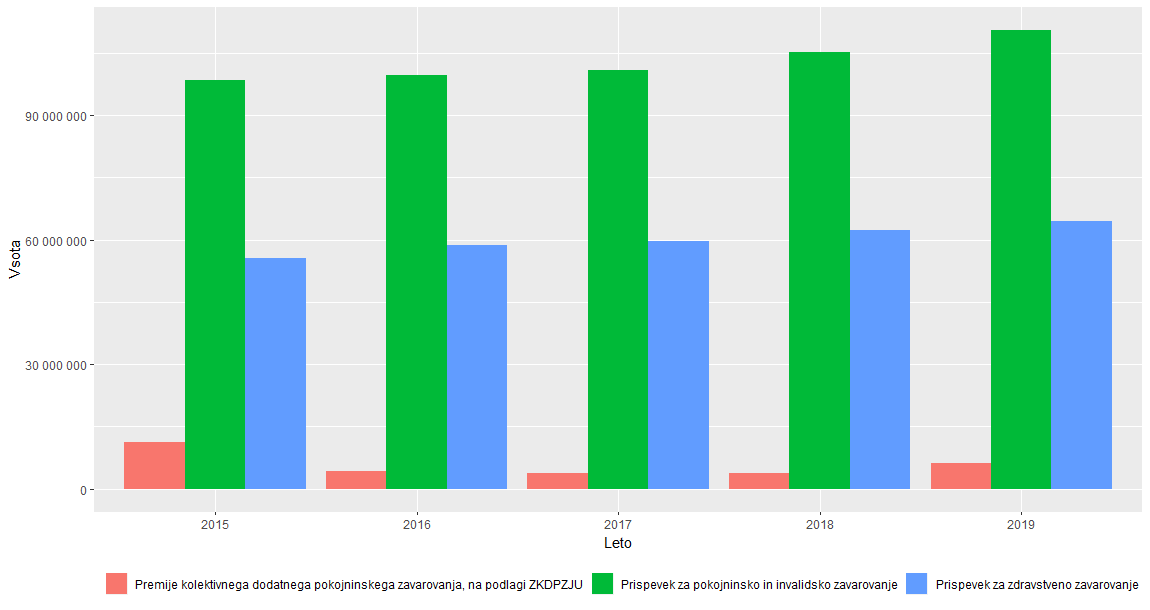
\includegraphics[width = 10 cm]{prispevki_delodajalcev_za_socialno_varnost_graf.png}
	\caption{Prispevki za pokojninski sklad v proračunu RS}
	\label{Slika 3}
	\end{figure}
\end {frame}

\begin{frame}
\subsubsection[Financiranje pokojnin iz državnega proračuna]{Financiranje pokojnin iz državnega proračuna}
	\frametitle{Financiranje pokojnin iz državnega proračuna}
	ZPIZ2 v dveh členih povzema naloge državnega proračuna pri financiranju pokojninskega zavarovanja, to sta 	člena 162. in 163.:
	\begin{itemize}
	\item \textbf{162. člen}: Sofinanciranje iz državnega proračuna: Republika Slovenija iz državnega proračuna in iz drugih virov zagotavlja sredstva za pokrivanje razlike med 				prihodki zavoda iz prispevkov in iz drugih virov ter odhodki zavoda.
	\item \textbf{163. člen}: Zagotavljanje likvidnosti zavoda: Če zavodu primanjkuje likvidnih sredstev za izpolnitev obveznosti za izplačilo pokojnin in drugih obveznosti 				ter za kritje morebitnega primanjkljaja med prihodki in odhodki v posameznem koledarskem letu, mu Republika Slovenija iz državnega proračuna zagotovi potrebna 				sredstva.
\end{itemize}

Pomembne novosti v dodatnem pokojninskem zavarovanju, s sprejetjem drugega zakona o  pokojninskem in invalidskem zavarovanju:
\begin{itemize}
	\item Vsi zaposleni so po svoji izbiri vključeni v kolektivno dodatno pokojninsko zavarovanje.
	\item Mlajšim zavarovancem bo zagotovljen manj konzervativen način varčevanja.
	\item Vključitev tudi samostojnih podjetnikov in pretežnih lastnikiov podjetja.
\end{itemize}
\end{frame}

\begin{frame}
\subsubsection[Demografska primerjava z drugimi državami]{Demografska primerjava z drugimi državami}
\frametitle{Demografska primerjava z drugimi državami}
\begin{figure}[h]
\centering
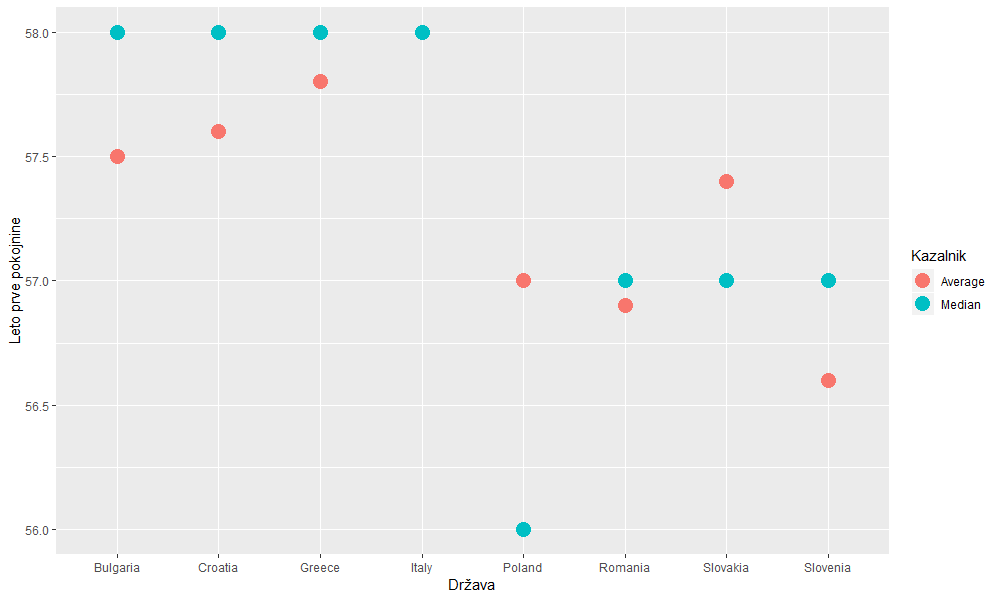
\includegraphics[height = 7 cm]{leto_prve_pokojnine.png}
\caption{Leto prve pokojnine}
\label{Slika 4}
\end{figure}
\end{frame}

\begin{frame}

\begin{figure}[h!]
\centering
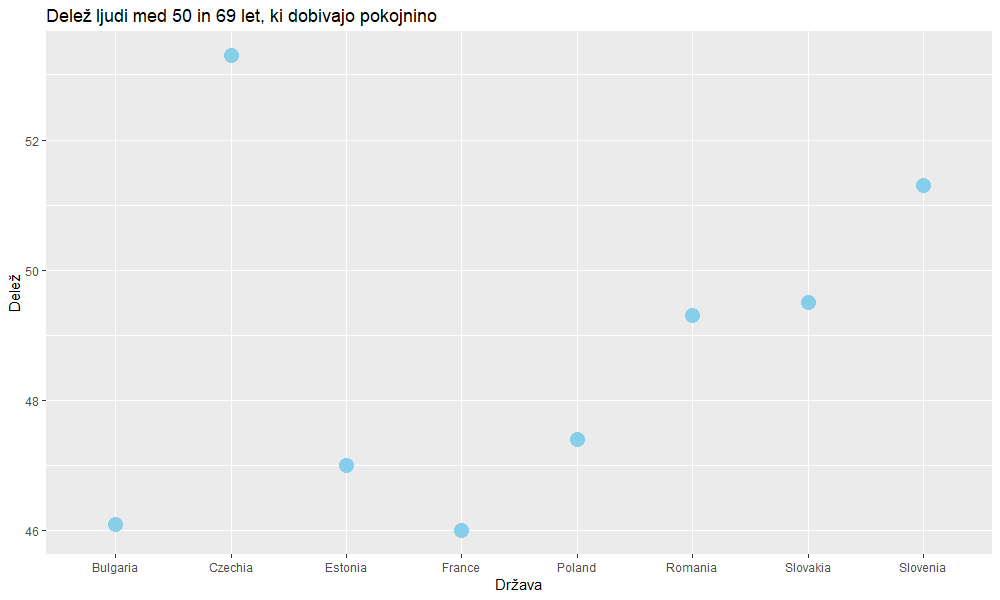
\includegraphics[width = 10 cm]{graf_procentualno_pokojnina.png}
\caption{Delež ljudi med 50 in 69 let, ki dobivajo pokojnino}
\label{Slika 5}
\end{figure}
\end{frame}



\begin{frame}
\subsubsection[Analiza pokojninskih transferjev v Sloveniji in ostalih državah]{Analiza pokojninskih transferjev v Sloveniji in ostalih državah}
\frametitle{Analiza pokojninskih transferjev v Sloveniji}
\begin{figure}[h!]
\centering
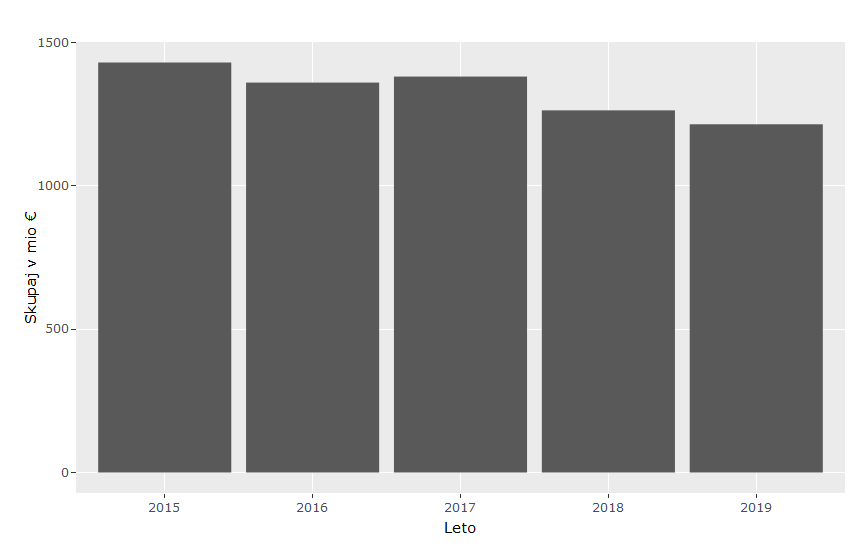
\includegraphics[width = 10 cm]{pokojnine_slovenija.png}
\caption{Pokojninski proračunski transferji}
\label{Slika 6}
\end{figure}
\end{frame}

\begin{frame}
\begin{figure}[h!]
\centering
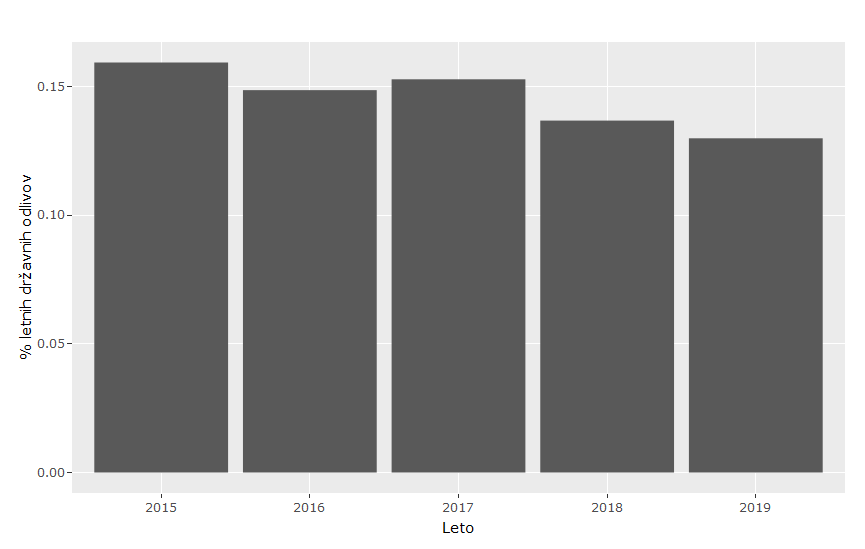
\includegraphics[width = 8 cm]{pokojnine_procentualno.png}
\caption{Delež proračunskih odhokov namenjen pokojninam}
\label{Slika 7}
\end{figure}

\begin{itemize}
\item država med leti 2015 in 2019 vsako leto nameni manj odhodkov za poravnavo pokojninskega računa
\item podatki na prvi pogled izgledajo ugodni, vendar nas rešuje ugodna gospodarska klima
\end{itemize}
\end{frame}

\begin{frame}
\frametitle{Posledice demografskih sprememb}
\begin{figure}[h!]
\centering
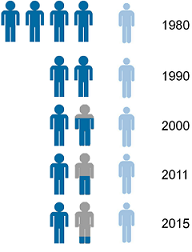
\includegraphics[width = 5 cm]{razmerje_med_zaposlenimi_in_upokojenimi_2015.png}
\caption{Razmerje med zaposlenimi in upokojenimi}
\label{Slika 8}
\end{figure}
\end{frame}


\begin{frame}
\frametitle{Analiza pokojninskih transferjev v drugih državah in primerjava s Slovenijo}
\begin{figure}[h!]
\centering
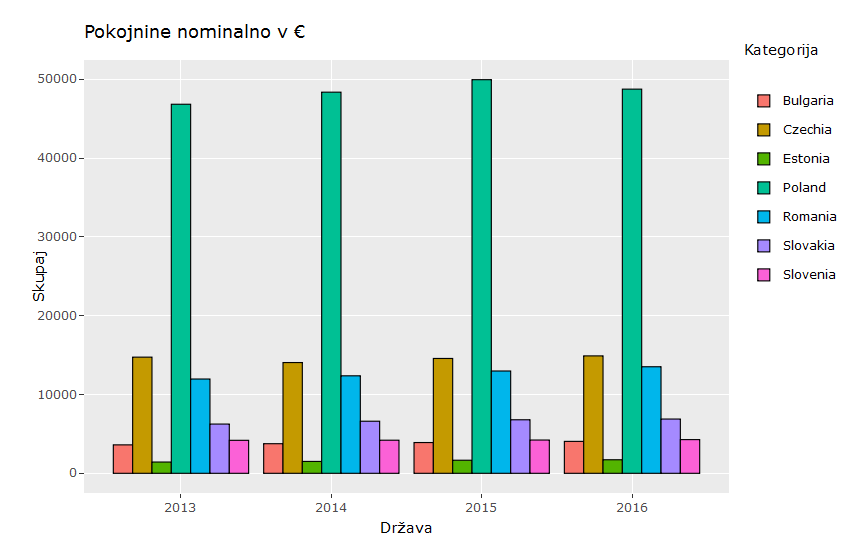
\includegraphics[width = 10 cm]{pokojnine_nominalno.png}
\caption{Nominalni pokojninski transferi v \euro}
\label{Slika 9}
\end{figure}
\end{frame}

\begin{frame}
\begin{figure}[h!]
\centering
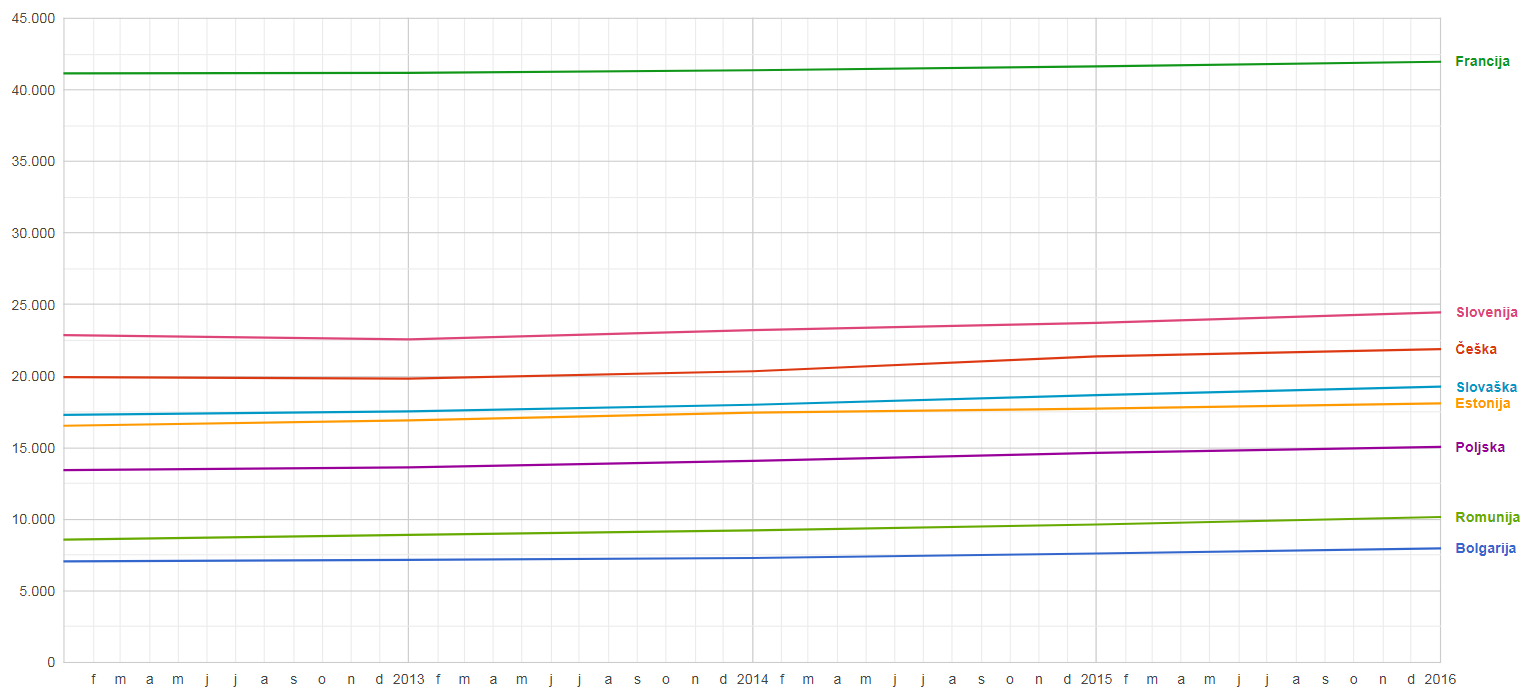
\includegraphics[width = 12 cm]{bdp_per_capita.png}
\caption{BDP na prebivalca}
\label{Slika 10}
\end{figure}
\end{frame}

\begin{frame}
\begin{figure}[h!]
\centering
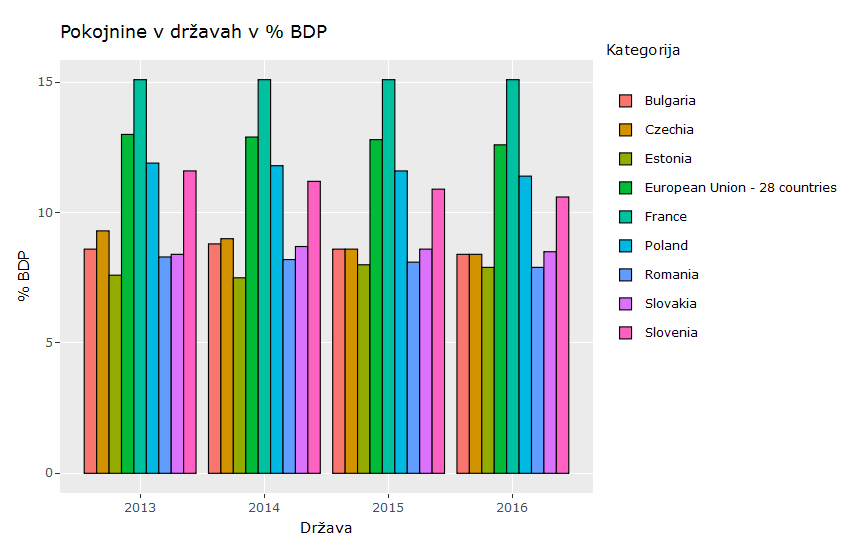
\includegraphics[width = 12 cm]{pokojnine_bdp.png}
\caption{Pokojnine v državah v \% BDP}
\label{Slika 11}
\end{figure}
\end{frame}


\begin{frame}
\subsection[Predolgi za spremembe pokojninskega sistema v Sloveniji]{Predlogi za spremembe pokojninskega sistema v Sloveniji}
\frametitle{Predlogi za spremembe pokojninskega sistema v Sloveniji}
Predlogi, ki so do neke mere že vključeni v pokojninskem sistemu:
\begin{itemize}
\item Spodbude za podaljšanje delovne dobe
\item Omejitev predčasnih upokojitev
\item Več sredstev iz dodatnega pokojninskega zavarovanja
\item Zaposlovanje starejših
\end{itemize}

\underline{ \textbf{Posledice sprememb:}}
\begin{columns}[T]
\begin{column}{0.5\textwidth}
\begin{block}{NEGATIVNE}
	\begin{itemize}
	\item zviševanje davka na delovno dobo
	\item dodatna izobraževanja za starejše
	\item napake in nenatančnost
	\item dodatni stroški bolniške odsotnosti
	\end{itemize}
\end{block}
\end{column}
\begin{column}{0.5\textwidth}  
\begin{block}{POZITIVNE}
	\begin{itemize}
	\item več delovnih izkušenj in določenega znanja
	\item prenos znanja na mlajše
	\item olajšava za DDPO - olajšava v višini 45\% plače te osebe
	\end{itemize}
\end{block}
\end{column}
\end{columns}
\end{frame}

\begin{frame}
\frametitle{Viri}
\section[Viri]{Viri}
\begin{itemize}
\item
\label{Splošno o proračunu}
\emph{Splošno o proračunu}, v: Ministrstvo za finance, [ogled 9.~4.~2019], dostopno na: \url{http://www.mf.gov.si/si/delovna_podrocja/proracun/splosno_o_proracunu/}.

\item
\label{Sestavni deli}
\emph{Sestavni deli proračuna}, v: Ministrstvo za finance, [ogled 9.~4.~2019], dostopno na: \url{http://www.mf.gov.si/si/delovna_podrocja/proracun/splosno_o_proracunu/sestavni_deli_proracuna/}.

\item
\label{Priprava proračuna}
\emph{Priprava proračuna}, v: Ministrstvo za finance, [ogled 9.~4.~2019], dostopno na: \url{http://www.mf.gov.si/si/delovna_podrocja/proracun/priprava_proracuna/}.

\item
\label{Izvrševanje proračuna}
\emph{Izvrševanje proračuna}, v: Ministrstvo za finance, [ogled 9.~4.~2019], dostopno na: \url{http://www.mf.gov.si/si/delovna_podrocja/proracun/izvrsevanje_proracuna/}.

\item
\label{Prebivalstvo Slovenije}
\emph{Prebivalstvo po letih}, v: Statistični urad Republike Slovenije, [ogled 22.~4.~2019], dostopno na: \url{https://pxweb.stat.si/pxweb/Dialog/viewplus.asp?ma=H132S&ti=&path=../Database/Hitre_Repozitorij/&lang=2}.
\end{itemize}
\end{frame}

\begin{frame}
\begin{itemize}
\item
\label{Eurostat pokojnine}
\emph{Age at which the person first received an old-age pension (years)}, v: Eurostat, [ogled 22.~4.~2019], dostopno na: \url{https://ec.europa.eu/eurostat/web/products-datasets/-/lfso_12agepens}.

\item
\label{Struktura prebivalstva}
\emph{List of countries by age structure}, v: Wikipedia, [ogled 22.~4.~2019], dostopno na: \url{https://en.wikipedia.org/wiki/List_of_countries_by_age_structure}.

\item
\label{Eurostat pokojnine procentualno}
\emph{Persons who receive a pension, by type of pension (\%)}, v: Eurostat, [ogled 22.~4.~2019], dostopno na: \url{https://ec.europa.eu/eurostat/web/products-datasets/-/lfso_12penstyp}

\item
\label{ZPIZ2}
\emph{Zakon o pokojninskem in invalidskem zavarovanju, IV. poglavje: PRIHODKI IZ DRŽAVNEGA PRORAČUNA}, v: Zakonodaja.com, [ogled 6.~5.~2019], dostopno na: \url{https://tinyurl.com/y4jutc7c}.

\item
\label{Novosti ZIPZ2}
\emph{Ključne novosti, ki jih na področju dodatnega pokojninskega zavarovanja uvaja ZPIZ-2}, v: Modra zavarovalnica, [ogled 6.~5.~2019], dostopno na: \url{https://www.modra-zavarovalnica.si/fileadmin/Javne_objave/Kljucne_novosti_ZPIZ-2.pdf}.
\end{itemize}
\end{frame}

\begin{frame}
\begin{itemize}
\item
\label{Dodatek na delovno dobo in drugi dodatki k plači}
\emph{Dodatek na delovno dobo in drugi dodatki k plači}, v: DATA, [ogled 8.~5.~2019], dostopno na:\\ \url{https://data.si/blog/2017/12/18/dodatek-na-delovno-dobo/?fbclid=IwAR1u_oxmL1oT8GC9yIIM2JWWowee2oL5lxf7BlAPviQYCoQYw6ZR8pGEilI}.



\item
\label{Pokojninski transferji v državah}
\emph{Pokojninski transferji v državah}, v: DATA, [ogled 9.~5.~2019], dostopno na: \url{http://appsso.eurostat.ec.europa.eu/nui/show.do?dataset=spr_exp_pens&lang=en}.

\item
\label{BDP na prebivalca}
\emph{BDP na prebivalca}, v: Google/World Bank, [ogled 9.~5.~2019], dostopno na: \url{https://www.google.com/publicdata/explore?ds=d5bncppjof8f9_&ctype=l&strail=false&bcs=d&nselm=h&met_y=ny_gdp_pcap_kd&scale_y=lin&ind_y=false&rdim=region&idim=country:SVN:SVK:BGR:CZE:EST:POL:FRA&ifdim=region&tstart=1336514400000&tend=1462744800000&hl=sl&dl=sl&ind=false&icfg}.

\item
\label{Razmerje med zaposlenimi in upokojenci}
\emph{Razmerje med zaposlenimi in upokojenci}, v: DATA, [ogled 9.~5.~2019], dostopno na: \url{https://www.modra-zavarovalnica.si/posamezniki/varcevanje-za-dodatno-pokojnino/pokojninski-sistem-v-sloveniji/}.
\end{itemize}


\end{frame}




\end{document}
